% -*- root: ../../DAT2-A423_Project_Report.tex -*-
\section{Implementation of a JPEG image}
Looking back to section \ref{sec:designJPEG} we can start implementing this into our steganography program \textit{Stegasaurus}.
Also we can refer to figure \ref{fig:JPEGprocess} for the steps the encoder must take.

There are multiple constructors to the \lstinline|JPEGImage| class, as a user can chose to specify custom Quantization- or Huffman tables, or simply use the default table which both the \lstinline|QuantizationTable|- and \lstinline|HuffmanTable| classes provides, by not providing any tables in the constructor.
The default tables in the respective classes are both found in the JPEG specification \citep[Annex k]{JPEGStandard}.

The \lstinline|void Encode(byte[])| is where the actual JPEG encoding takes place.
The method can be seen in listing \ref{JPEGEncode}.
The most significant part of the JPEG file is obviously the scan data, but before that can be written to the file, we have to encode most of the headers first.
We do that by calling \lstinline|void _writeHeaders()|.
All information needed in these headers are already known, as both the bitmap image and tables provided in the constructor.

\begin{lstlisting}[firstnumber=136,label=JPEGEncode]
public void Encode(byte[] message) {
    //Instantiate a JpegWriter, which has an internal list of bytes 
    //and the logic required to write those to a file
    _jw = new JpegWriter();

    if (message.Length > 16884) {
        throw new ArgumentException("Message cannot be longer than 16884 bytes!");
    }
    _breakDownMessage(message);

    _writeHeaders();
    _writeScanData();
    _writeEndOfImage();
}
\end{lstlisting}

From here on, we need to perform all of the regular steps JPEG encoding up until just before the Huffman encoding.
We start out with splitting the image into Y, Cb and Cr channels instead of the \lstinline|Bitmap|'s RGB channels, and then in the method \lstinline|void _encodeAndQuantizeValues(sbyte[][,], int, int)| we have the loop which can be seen in listing \ref{JPEGEncodeAndQuantize}.
While these nested loops may seem very computationally heavy, what it actually does is that it loops through the three channels of every pixel in the 16x16 MCU's.
So while we have five nested for loops, we only run through every pixel 3 times. After every 16x16 MCU has been filled with values, the MCU must be encoded. As the name Minimum Encoded Unit implies, we can encode one MCU without depending on the other. That means that after we fill one MCU, we can encode that directly, we do that by invoking the method \lstinline|void _encodeBlocks(float[][,])|

\begin{lstlisting}[firstnumber=525, label=JPEGEncodeAndQuantize]
for (int MCUY = 0; MCUY < imageHeight; MCUY += 16) {
    for (int MCUX = 0; MCUX < imageWidth; MCUX += 16) {
        for (int i = 0; i < 3; i++) {
            for (int x = 0; x < 16; x++) {
                for (int y = 0; y < 16; y++) {
                    channels[i][x, y] = YCbCrChannels[i][MCUX + x, MCUY + y];
                }
            }
        }
        _encodeBlocks(channels);
    }
}
\end{lstlisting}

In this method, we split the MCU into 8x8 blocks. As we have a fixed sampling of 4:2:0 that means that we split the Y channel into four 8x8 blocks and effectively save all information about the luminance channel, the Cr and Cb channels, we down-sample from a 16x16 block to a 8x8 blocks. As we implemented this, we had two ways of doing so. One way of doing it, is taking every 4th value in the block as seen on figure \ref{fig:downsampling4th}, and the other way of doing it, is taking an average of each 2x2 block in the 16x16 MCU as seen on figure \ref{fig:downsamplingAverage}.

\begin{figure}
    \centering
    \begin{subfigure}[b]{0.3\textwidth}
        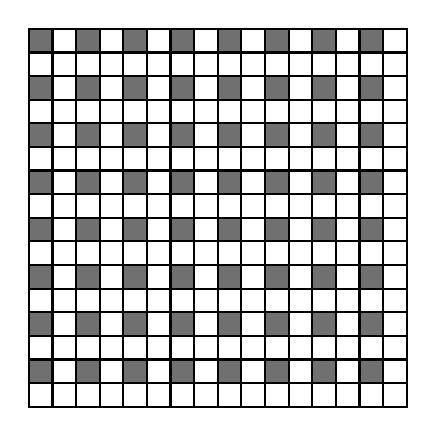
\begin{tikzpicture}
    [%%%%%%%%%%%%%%%%%%%%%%%%%%%%%%
        box/.style={rectangle,draw=black,thick, minimum size=0.3cm},scale=0.3
    ]%%%%%%%%%%%%%%%%%%%%%%%%%%%%%%

\foreach \x in {0,1,...,15}{
    \foreach \y in {0,1,...,15}
        \node[box] at (\x,\y){};
}

\foreach \x in {0,2,4,6,8,10,12,14}{
    \foreach \y in {1,3,5,7,9,11,13,15}
        \pgfmathparse{44}
        \edef\tmp{\pgfmathresult}
        \node[box,fill=white!\tmp!black] at (\x,\y){};
} 

\end{tikzpicture}
        \caption{Downsampling by choosing only every 4th value}
        \label{fig:downsampling4th}
    \end{subfigure}
    \qquad %add desired spacing between images, e. g. ~, \quad, \qquad, \hfill etc. 
      %(or a blank line to force the subfigure onto a new line)
    \begin{subfigure}[b]{0.3\textwidth}
        \begin{tikzpicture}
    [%%%%%%%%%%%%%%%%%%%%%%%%%%%%%%
        box/.style={rectangle,draw=black,thick, minimum size=0.6cm},scale=0.6
    ]%%%%%%%%%%%%%%%%%%%%%%%%%%%%%%

\foreach \x in {0,1,...,7}{
    \foreach \y in {0,1,...,7}
        \node[box] at (\x,\y){};
}
\foreach \x in {0,1,...,7}{
    \foreach \y in {0,1,...,7}
        \pgfmathparse{\intcalcMod{\x}{2} * 22 + \intcalcMod{\y}{2} * 22 + 22}
        \edef\tmp{\pgfmathresult}
        \node[box,fill=white!\tmp!black] at (\x,\y){};
}

\end{tikzpicture}
        \caption{Downsampling by taking an average of every four values}
        \label{fig:downsamplingAverage}
    \end{subfigure}
    \caption{Different methods for downsampling of 16x16 MCU to an 8x8 block}\label{fig:downsampling}
\end{figure}








\subsection{Working with bits}
While working with JPEG images, bit-patterns and bit-wise operations often occur.
Due to hardware limitations, a single bit in the memory cannot be changed individually, and we can only address the individual bytes.
There are now two ways that we can go about this:
Either we use bytes to represent bits, and effectively waste 7 bits of memory for each bit, or we use the class \lstinline|BitArray| from the \lstinline|System.Collections| library.
What this class does, is that it handles the packing of the bits into bytes, and makes you able to adress the individual bits.

The \lstinline|BitArray| seemed like the way to go, and we implemented a class \lstinline|BitList| which implemented List-like features like \lstinline|Add| and \lstinline|Insert| while using the \lstinline|BitArray| to store our data.
The implementation can be seen in appendix \ref{app:C}. 

The \lstinline|BitArray| offers the functionality of modifying the length of the array, so that more values can be added.
This means that every time the \lstinline|BitList| runs out of space in the underlying \lstinline|BitArray|, we simply multiply the length of the array by 2, so that more values can be added.
This makes appending to the array relatively fast, since we have enough room to add more values most of the time.
Inserting values in the middle of the array proved to be much more difficult, however.

When inserting a value into the array, all values after the value to be inserted have to be shifted, so that room is made from the new value.
In an example 512x512 image, we have over 750,000 bits to save, and if we were to insert a bit in the beginning of the array, we would have to move 750,000 elements in the array.
All in all a very computationally expensive operation.

So while the \lstinline|BitArray| seemed promising in theory, saving us a lot of memory, the need of inserting bits into the middle of the array makes using the \lstinline|BitArray| infeasible.
What we need to solve this problem is to eliminate the need to shift a large part of the array. 
One way of solving this problem is to make a data type which combines the functionality of the \lstinline|BitArray| with a linked list. 
By splitting up the large \lstinline|BitArray| into smaller linked arrays we could shift the values in the smaller arrays. 
We would have a slightly longer access time, but have a much faster insertion time. 
Another way to solve the problem, and what we ended up doing was to eliminate the need of inserting the values. 
We realised that the only time we need to insert values into the \lstinline|BitList| was when there were 8 consecutive ones in the scan data. 
So what we did what created the method \lstinline|CheckedAdd| which we would use while writing scan data to the list. 
This method would then keep track of the last inserted values, and insert the zeroes on-the-fly instead of after the whole process. 
The method \lstinline|CheckedAdd| can also be seen in appendix \ref{app:C}